\documentclass[ 12pt, xcolor=beamer,table,usenames,dvipsnames, ignorenonframetext, ngerman]{beamer}
\usetheme{Frankfurt}
\usecolortheme{dove}
\usepackage{appendixnumberbeamer}
%\setbeamersize{text margin left=20pt,text margin right=20pt,}
\useoutertheme{miniframes}
\beamertemplatenavigationsymbolsempty 
\setbeamertemplate{mini frames}{}
\setbeamertemplate{itemize item}{\textbullet}

\addtobeamertemplate{navigation symbols}{}{
	\ifnum\insertframenumber>\inserttotalframenumber%
	\relax
	\else%
	\usebeamerfont{footline}%
	\usebeamercolor[fg]{footline}%
	\hspace{1em}%
	\insertframenumber
	\fi%
}
\setbeamercolor{footline}{fg=black}
\setbeamercolor{palette primary}{bg=blue!15,fg=black}
\setbeamercolor{background canvas}{bg=blue!5}
\setbeamercolor{palette secondary}{bg=blue!5}
\setbeamercolor{palette tertiary}{bg=blue!5}
\setbeamercolor{palette quaternary}{bg=blue!5}
\usepackage{soul}
\makeatletter
\let\HL\hl
\renewcommand\hl{%
	\let\set@color\beamerorig@set@color
	\let\reset@color\beamerorig@reset@color
	\HL}

\usepackage{tipa}
\usepackage{tikz}
\usetikzlibrary{shapes.geometric, arrows}
\mode<presentation>

\setbeamercovered{invisible}
\usepackage{multicol}
\usepackage[english]{babel}
\usepackage[latin1]{inputenc}
\usepackage{times}
\usepackage[T1]{fontenc}
\usepackage{ulem}
\usepackage{tipa}
\usepackage{qtree}
\usepackage{phonrule}
\usepackage{graphicx}
\usepackage{apacite}
\usepackage{xcolor}
\setlength\parindent{0pt}
\usepackage{natbib}
\usepackage{tikz}
\usetikzlibrary{arrows.meta}
\usepackage{tcolorbox}
\tcbuselibrary{raster}

\DeclareRobustCommand{\greencheck}{%
	\tikz\fill[scale=0.6, color=ForestGreen]
	(0,.35) -- (.25,0) -- (1,.7) -- (.25,.15) -- cycle;%
}
\title{Extending communication games to more players}
\author{Veronica Boyce}
\date{LangCog Lab Meeting}
\begin{document}

\begin{frame}
\maketitle
\pause
\begin{tikzpicture}[remember picture,overlay]
\node[xshift=1.5cm,yshift=1.2cm] at (current page.south west) {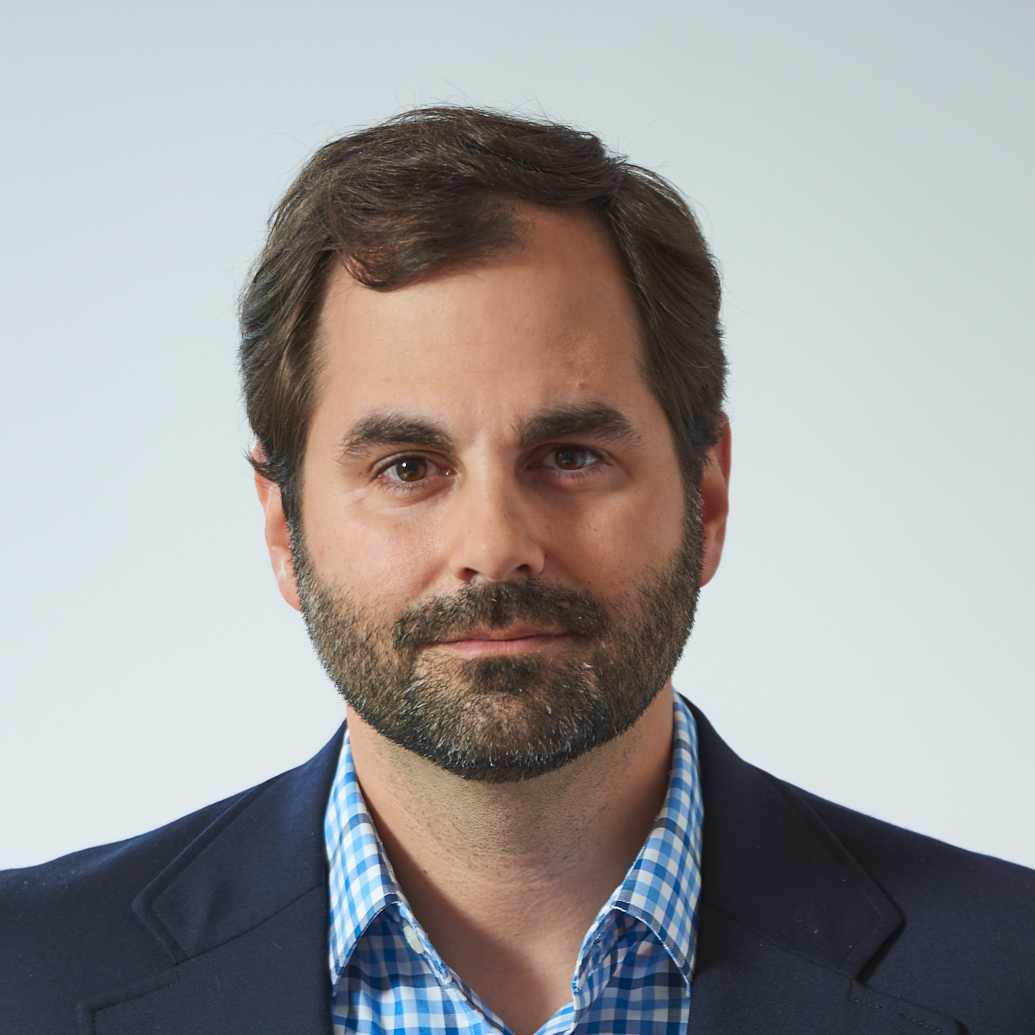
\includegraphics[width=.2\textwidth]{../images/mike.jpg}};
\node[xshift=-2.5cm,yshift=1.2cm] at (current page.south) {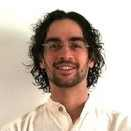
\includegraphics[width=.2\textwidth]{../images/noah.jpg}};
\node[xshift=0cm,yshift=1.2cm] at (current page.south) {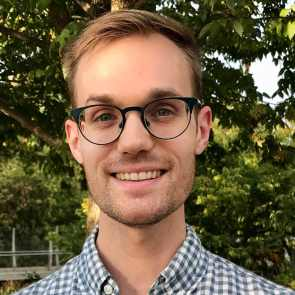
\includegraphics[width=.2\textwidth]{../images/robert.jpeg}};\pause
\node[xshift=-2.5cm,yshift=1.2cm] at (current page.south east) {
\includegraphics[width=.4\textwidth]{../images/hai.jpg}};
\end{tikzpicture}
\end{frame}


\begin{frame}{Why study communication?}
	\pause
	Verbal communication is a key method of human interaction.\\ \pause
	% share ideas, teach each other, 
	We communicate and understand more than surface meaning.\\ \pause
	
	Some of this is conventionalized, but some is dynamic. \\
	
%	Verbal communication is a key part of human interaction: we use it to ask for objects, teach
%	facts to others, and express our feelings. We tailor our communication depending on who we are
%	talking to according to our prior interactions with them, what words they know, and what they know
%	about the topic being discussed. This adaptation is dynamic; over the course of a conversation,
%	shared terminology and shorthands naturally arise.
	
\end{frame}

\begin{frame}{Partner-specific adaptation}
	\pause
	How is alignment achieved? 
	
	\pause
	Theoretical angles: \pause
	\begin{itemize} 
		\item Mental modelling (ex. RSA) (Clark \& Wilkes-Gibbs 1986, Goodman \& Frank 2016) \pause
		\item Interactive Alignment Account -- bottom up priming (Garrod \& Pickering 2009) \pause
		\item Audience Design (Yoon \& Brown Schmidt 2019)
	\end{itemize}
\end{frame}

%
\begin{frame}{Clark \& Wilkes-Gibbs 1986}
	
		%\item How do people coordinate in a conversation? 
		%People don't cleanly take turns, don't use full utterances, can do lots of confirmation or repair. 
	%	\item Reference as a microcosm 
		% counter to idealized linguistic or philosophical models, it's messy
	%	\item Tangram reference game has earlier antecedents, but this is foundational to reference coordination, conversational pacts
	%	\item Originates using *this* set of tangrams
		%\item Ordering task, 12 tangrams x 6 rounds, oral communication
	%	\item Timed and transcribed
	%	\item 8 dyads play a reference game
	%	\item Number of words declines over trials steeply between 1 \& 2 and then asymptotes
	%	\item Number of turns also declines
	%	\item Referents become more definite, less hedged
	%	\item Lots of qualitative descriptions
	\pause
	\vspace{-.2cm}
\begin{center}
	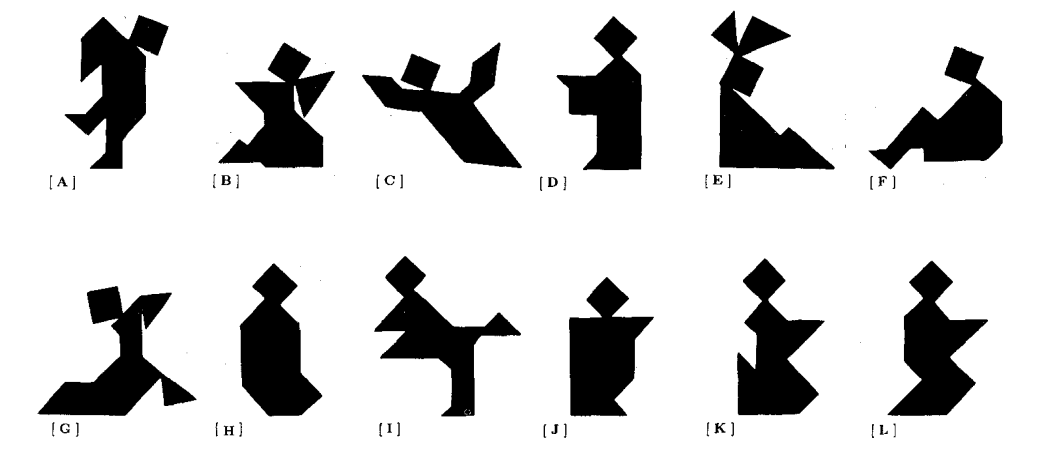
\includegraphics[width=.7\textwidth]{../images/clark_tangrams.png}
	\end{center}
\vspace{-.4cm}
\pause
\begin{small}
\begin{enumerate}
	\setlength{\itemsep}{-2pt}

	\item All right, the next one looks like a person who's ice skating, except, they're sticking two arms out in front. \pause
	\item Um, the next one's the person ice skating that has two arms? \pause
	\item The fourth one is the person ice skating, with two arms. \pause
	\item The next one's the ice skater. \pause
	\item The fourth one's the ice skater. \pause
	\item The ice skater.
	\end{enumerate}
\end{small}
\end{frame}

\begin{frame}{Clark \& Wilkes-Gibbs 1986}
	
	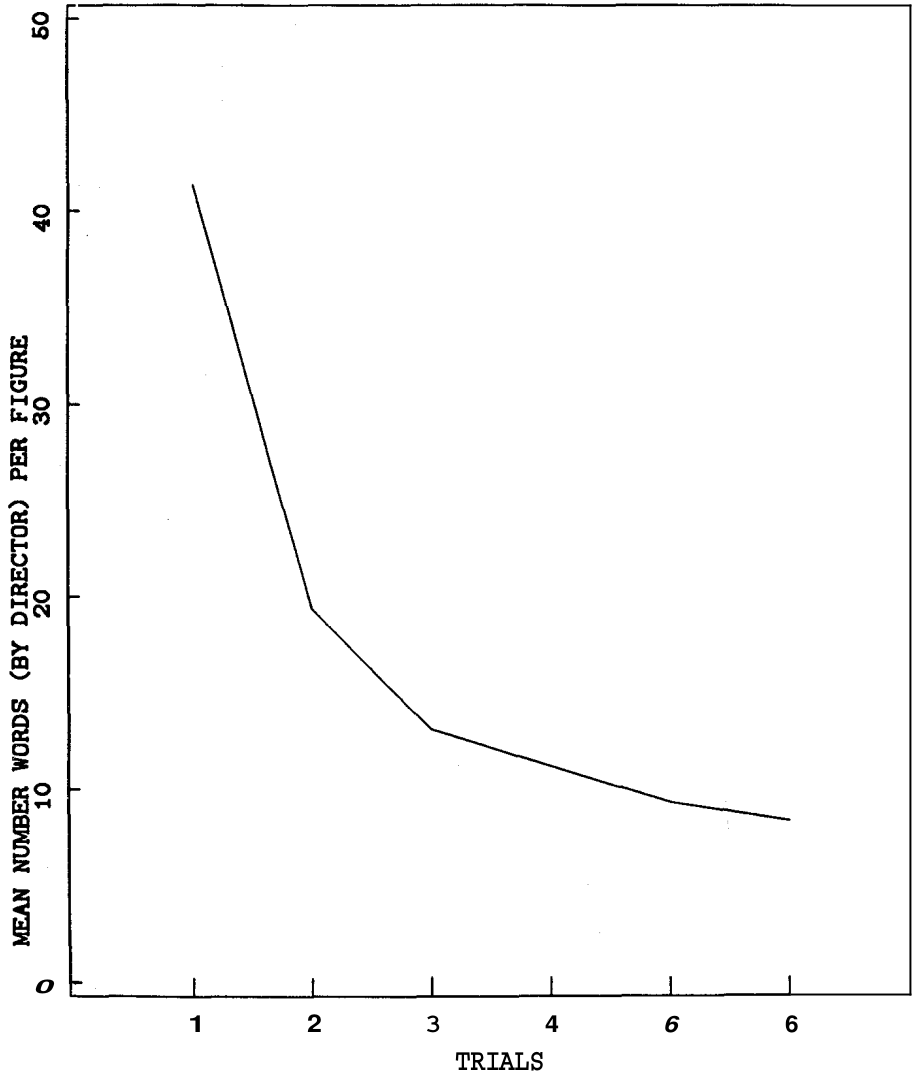
\includegraphics[width=.48\textwidth]{../images/clark_words.png}
		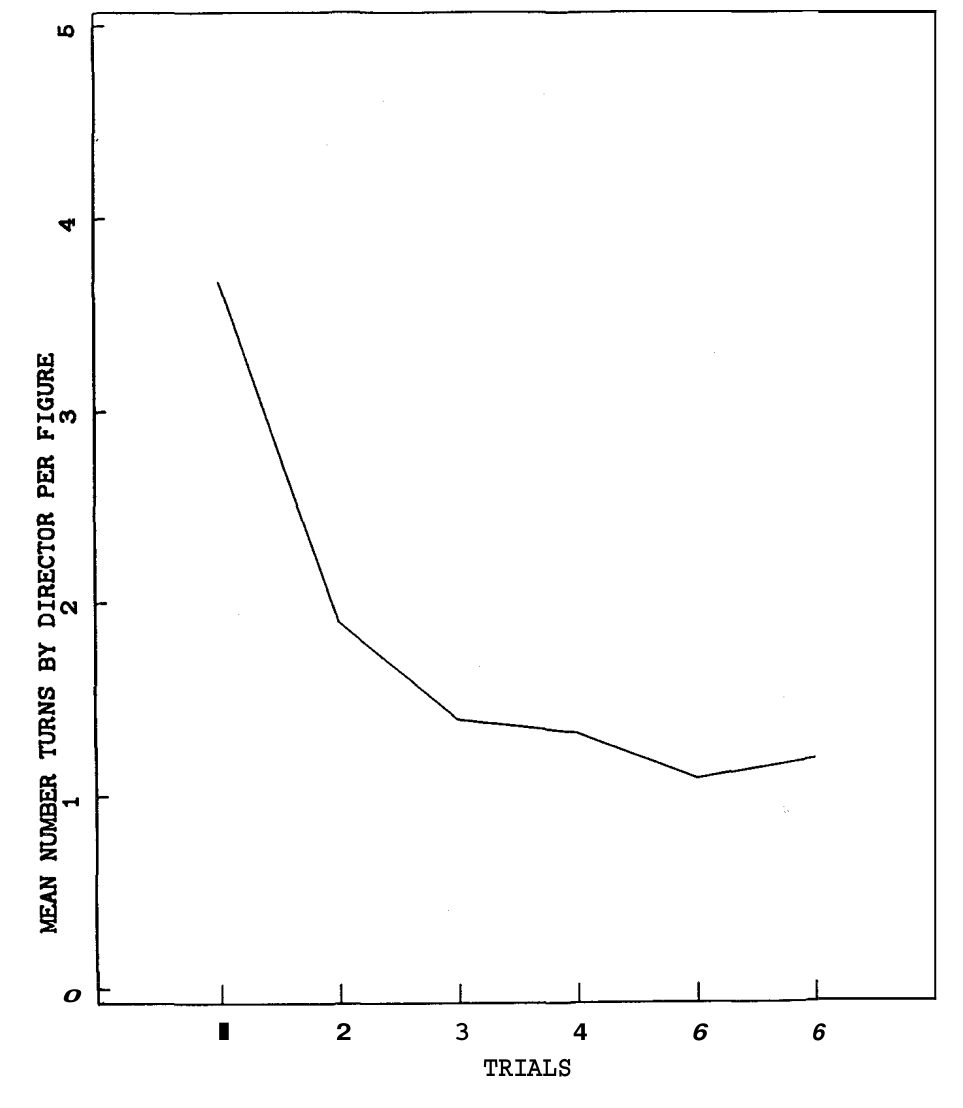
\includegraphics[width=.5\textwidth]{../images/clark_turns.png}	
		
\end{frame}
%
\begin{frame}{Hawkins, Frank, \& Goodman 2020}
Scaling up with web-based experiments
\begin{itemize}
	\item Cued version with feedback on each trial \pause
	\item Message with a chat box \pause
	\item After all exclusions, 83 dyads \pause
\end{itemize}
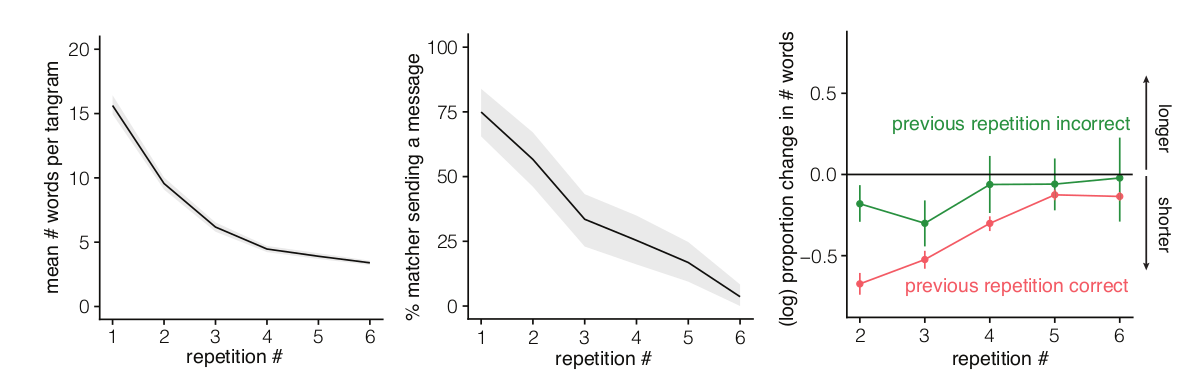
\includegraphics[width=\textwidth]{../images/hawkins_fewer_words.png}
\end{frame}
%
\begin{frame}{Hawkins, Frank, \& Goodman 2020}
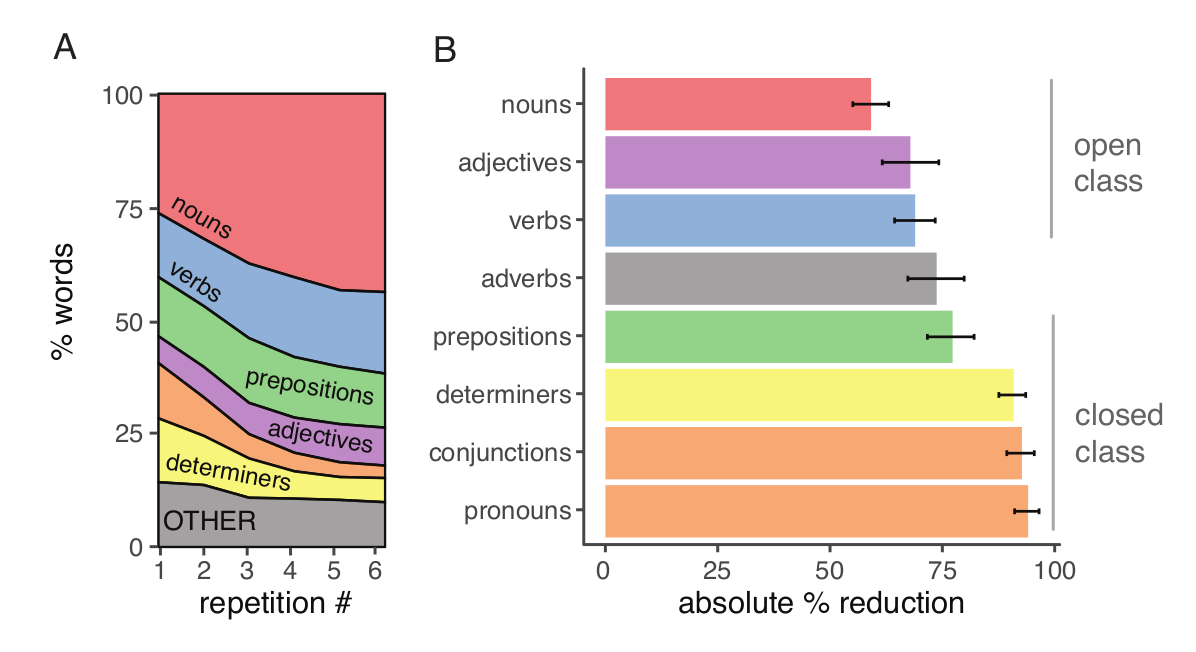
\includegraphics[width=\textwidth]{../images/hawkins_pos.png}
Words tend to drop out in syntactic units
\end{frame}

\begin{frame}{Hawkins, Frank, \& Goodman 2020}
	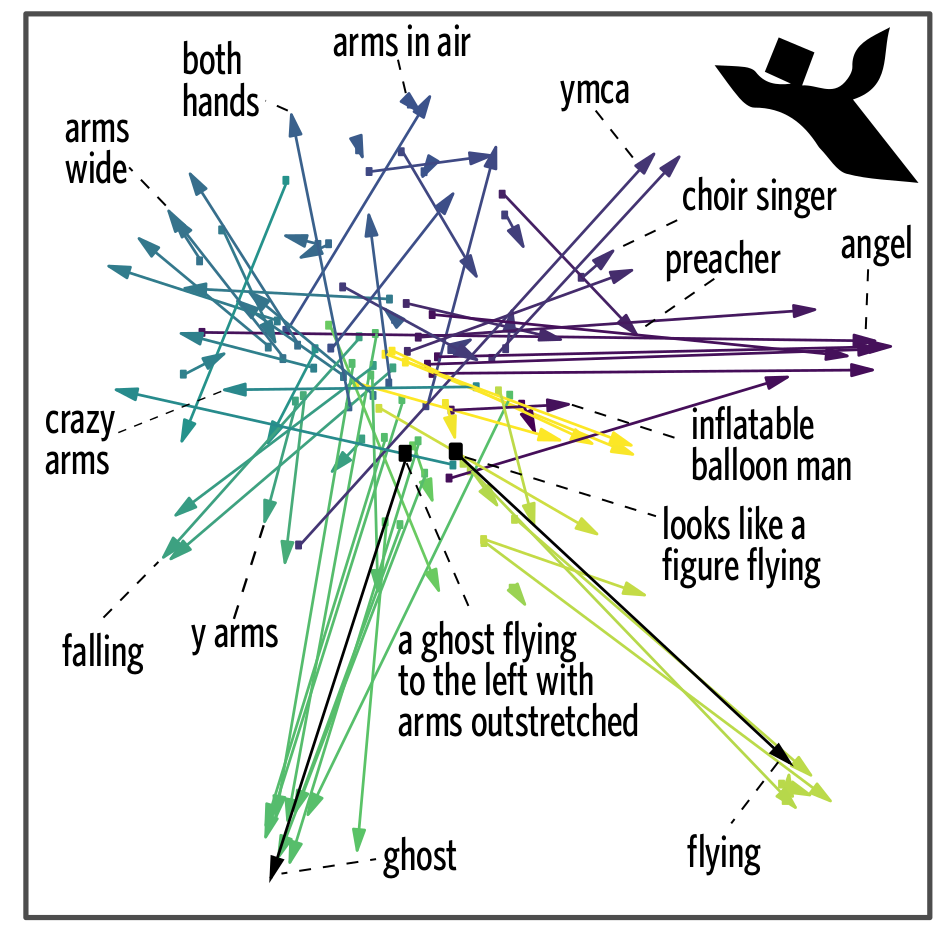
\includegraphics[width=.6\textwidth]{../images/hawkins_semantics.png}
	
	Semantics converge within and diverge between groups
\end{frame}


\begin{frame}{Yoon \& Brown-Schmidt 2019}
	Speaker talks to multiple matchers \\
	
	
	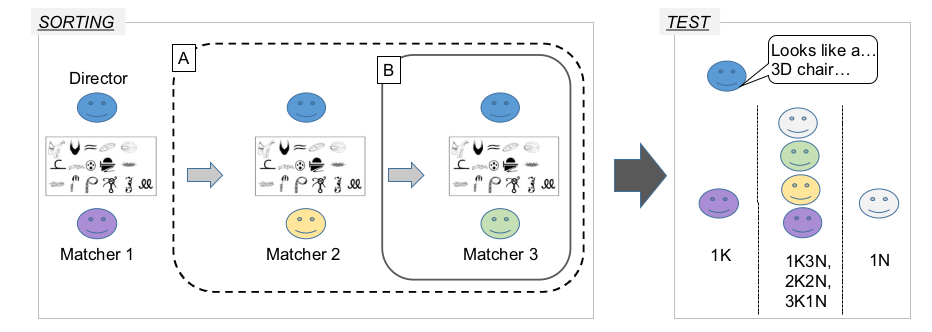
\includegraphics[width=\textwidth]{../images/yoon_diagram.png}
	
	Examine speaker's utterance length, elaborations, disfluencies
	%length, elaboration, disfluencies
\end{frame}
%
\begin{frame}{First Year Project}
	Dynamics of pact formation in larger groups \pause
	
	Compare groups of 2/3/4 communicators
	\begin{itemize}
		\item Look for differential reduction \pause
	\end{itemize} 
Rotate who is the knowledgeable speaker
\begin{itemize}
	\item Chosen for participant experience
	\item Stronger measure of alignment
\end{itemize}

\end{frame}

\begin{frame}{Experiment Framework}
Implemented in Empirica (Almaatouq et al 2020) 
 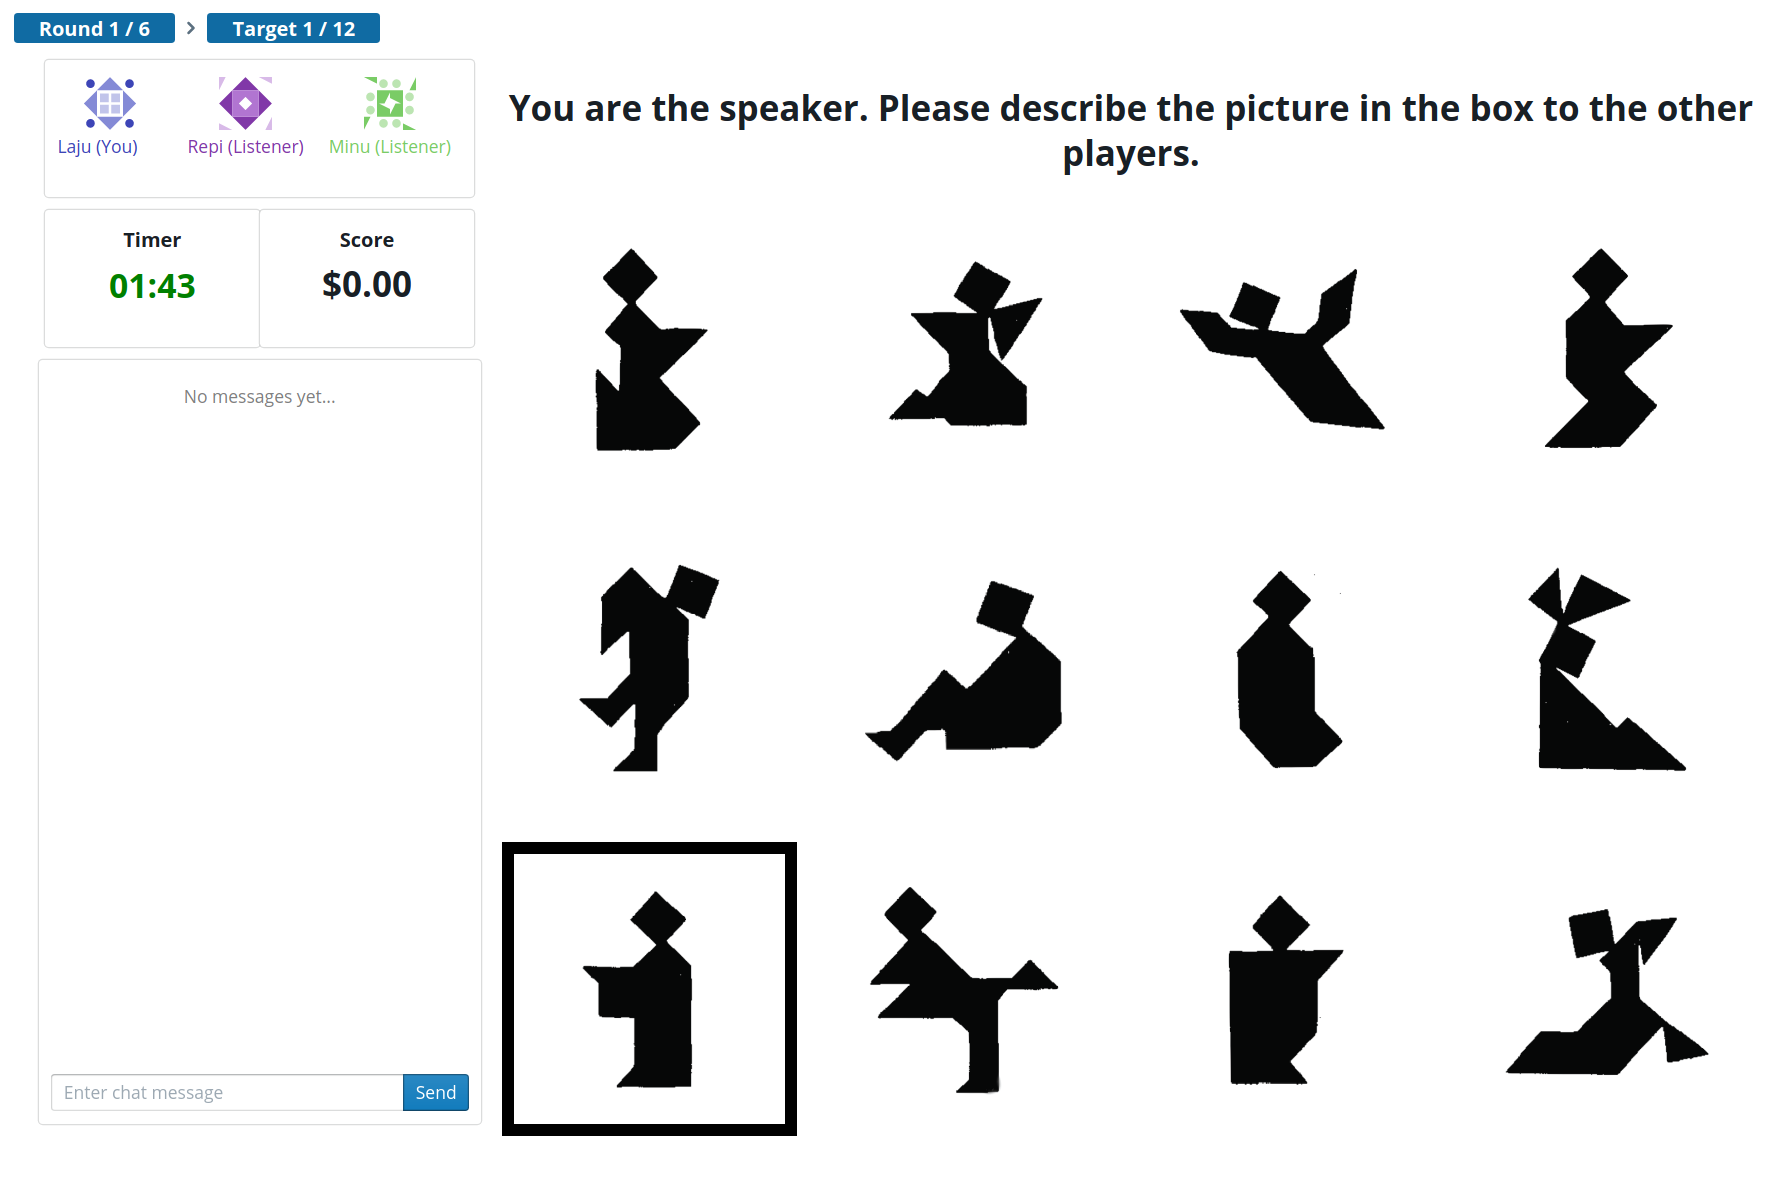
\includegraphics[width=.9\textwidth]{../images/interface.PNG}
\end{frame}

\begin{frame}{Experiment Framework}
	\only<1>{\begin{tikzpicture}[remember picture,overlay]
	\node[yshift=-.5cm] at (current page.center) {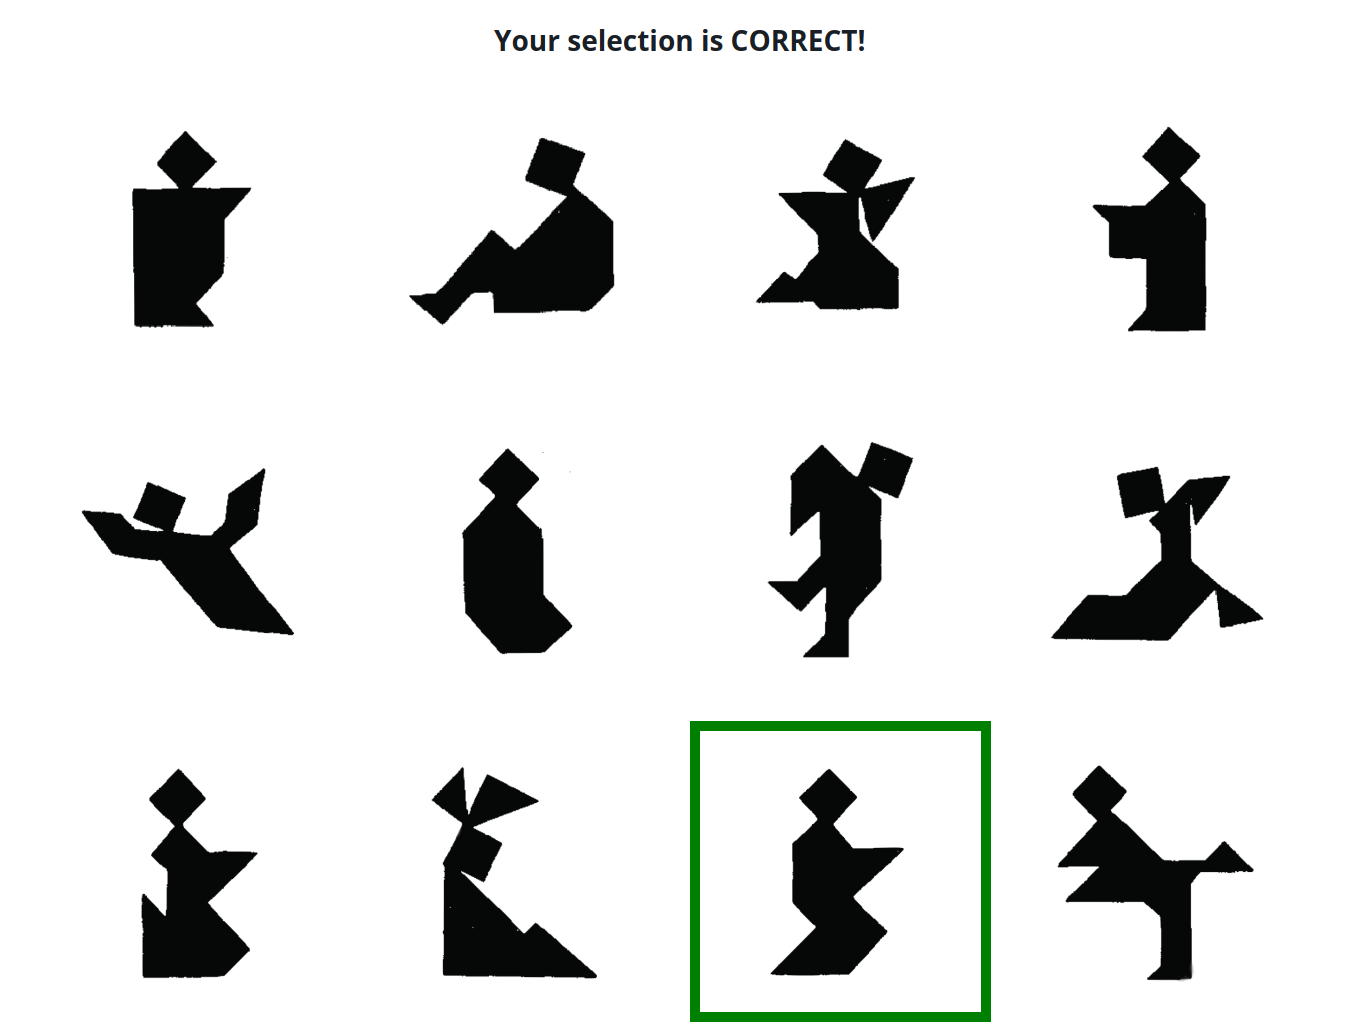
\includegraphics[width=.7\textwidth]{../images/listener_correct.png}};
		\node[yshift=1cm] at (current page.south) {Bonus: 4 points};
		\end{tikzpicture}}
\only<2>{\begin{tikzpicture}[remember picture,overlay]
\node[yshift=-.5cm] at (current page.center) {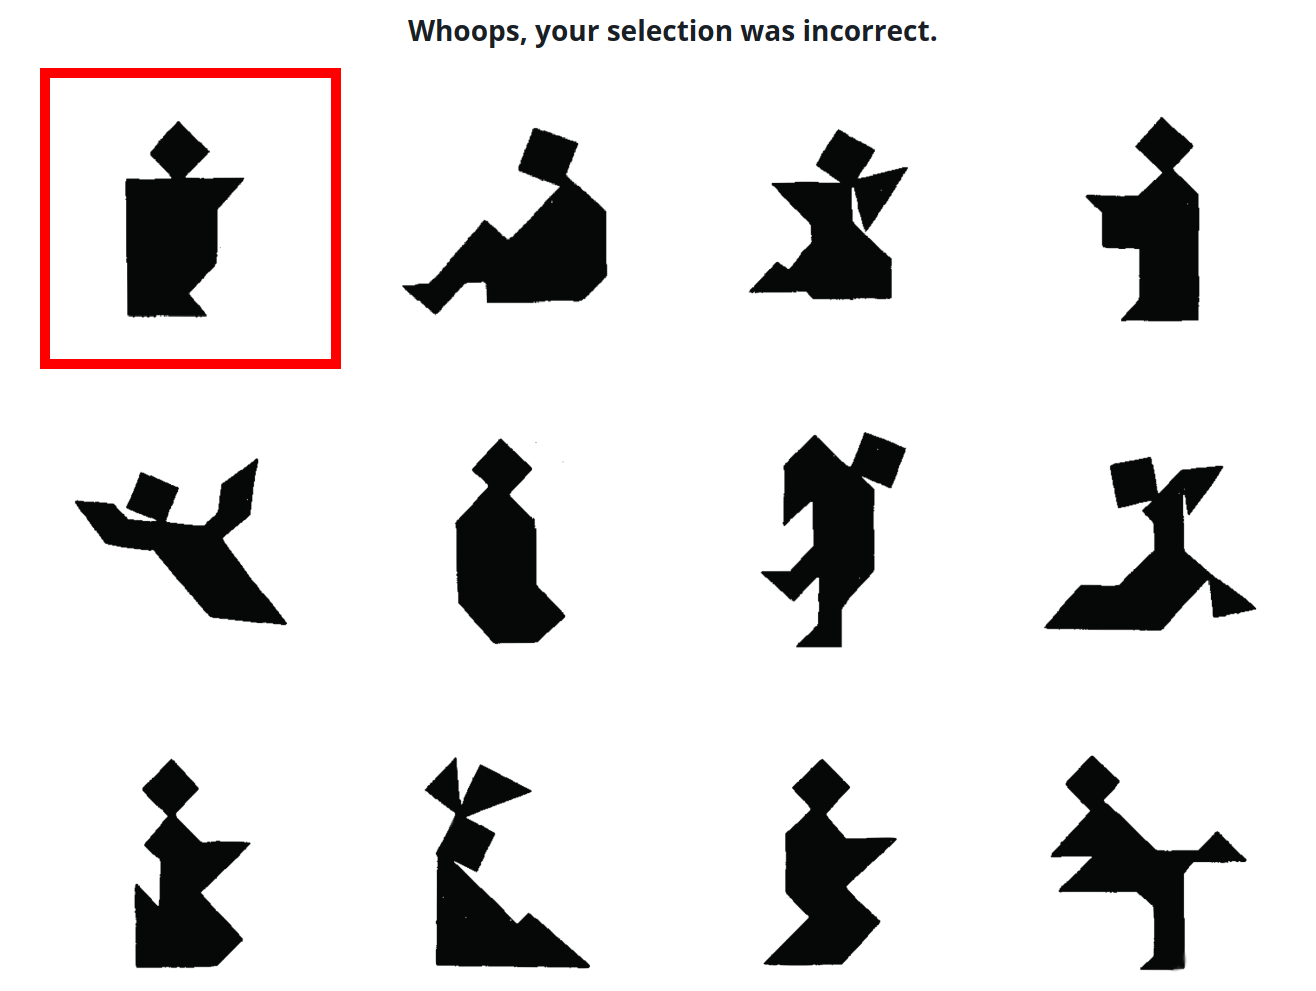
\includegraphics[width=.7\textwidth]{../images/listener_wrong.png}};
			\node[yshift=1cm] at (current page.south) {Bonus: 0 points};
			\end{tikzpicture}}
\only<3>{\begin{tikzpicture}[remember picture,overlay]
	\node[yshift=-.5cm] at (current page.center) {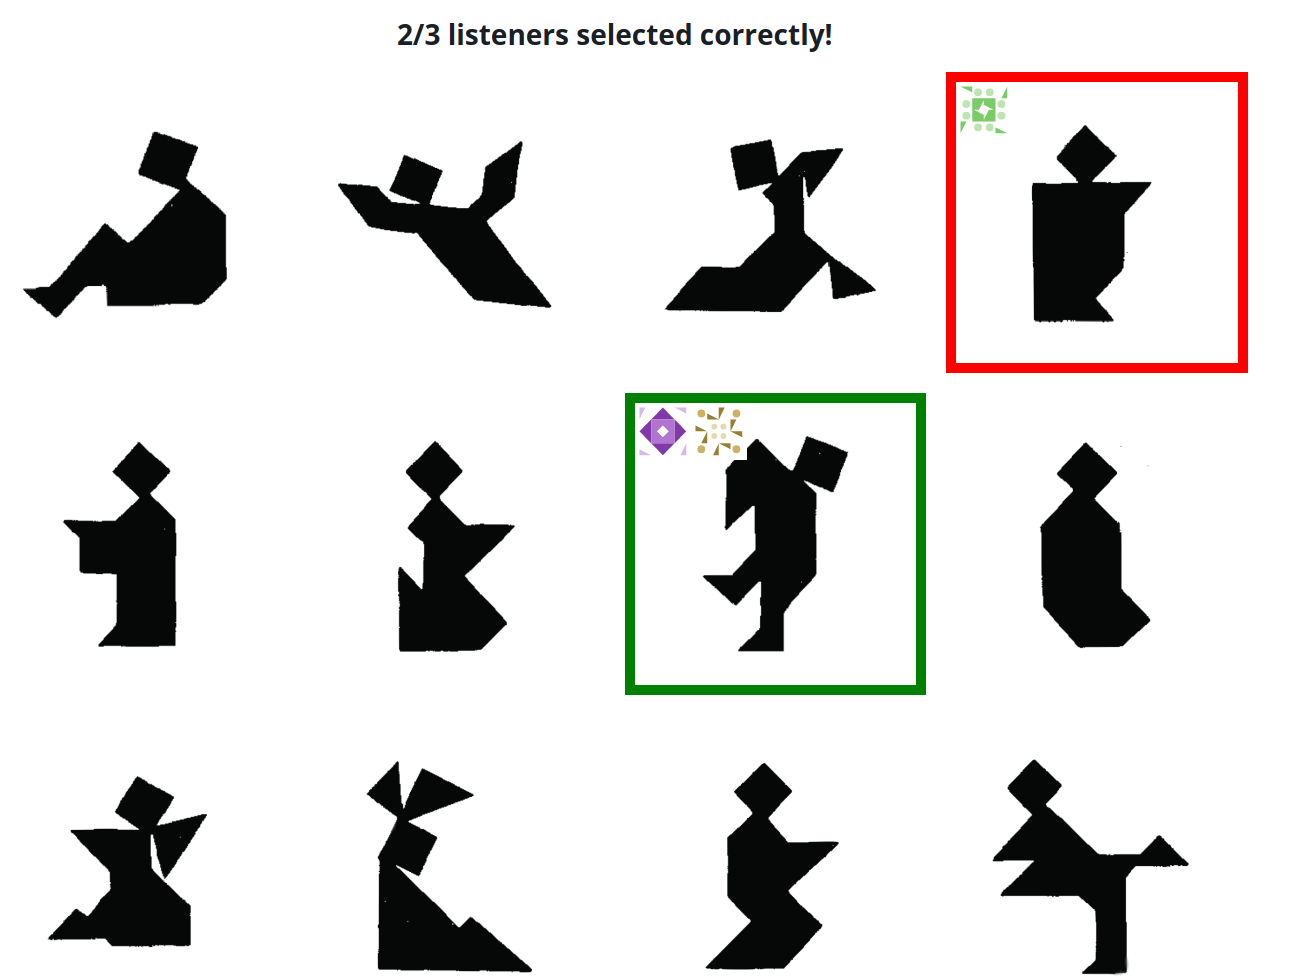
\includegraphics[width=.7\textwidth]{../images/speaker_feedback.png}};
\node[yshift=1cm] at (current page.south) {Bonus: Average of listeners = (2/3) * 4 points};

	\end{tikzpicture}}
\end{frame}
\begin{frame}{Recruitment}
	Goal: 20 games in each of 2/3/4 player 
	
	Each game has 6 blocks of 12 tangrams
	\medskip
	
	Actual recruitment:
	\begin{itemize}
		\item 15 2-player games (+ 4 partial)
		\item 18 3-player games (+ 2 partial)
		\item 20 4-player games (+ 1 partial)
	\end{itemize}
Include all complete blocks

\end{frame}


\begin{frame}{Results -- Accuracy}
	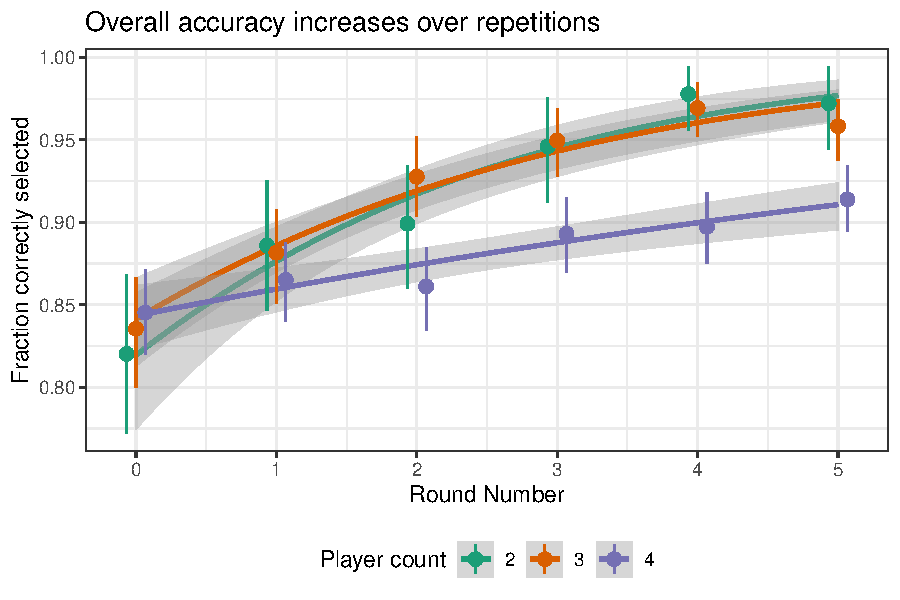
\includegraphics[width=\textwidth]{../images/accuracy.pdf}
	Accuracy is high and increasing
\end{frame}

\begin{frame}{Results -- Speed}
	
	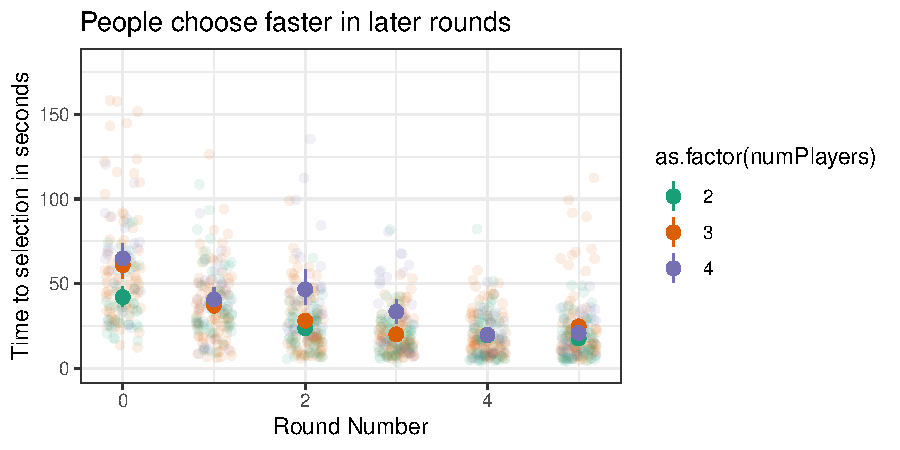
\includegraphics[width=\textwidth]{../images/time.pdf}
	Listeners choose faster in later rounds

\end{frame}

\begin{frame}{Reduction}
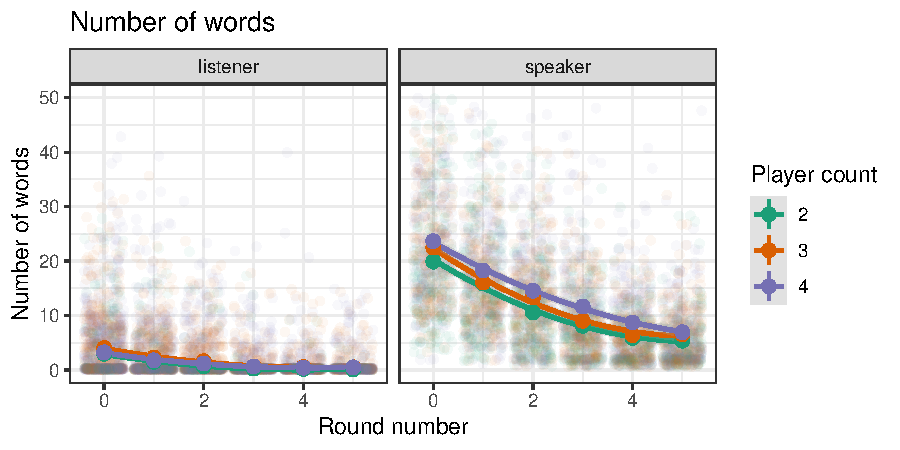
\includegraphics[width=\textwidth]{../images/words.pdf}
Number of words reduces over rounds
Caution: Non-referential utterances not yet removed
\end{frame}

\begin{frame}{Reduction}
	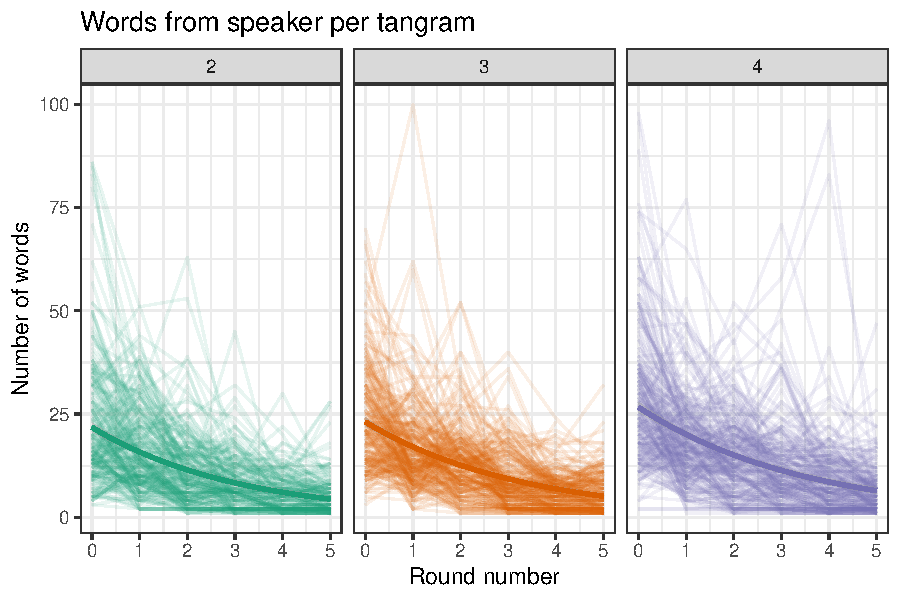
\includegraphics[width=\textwidth]{../images/words_lines.pdf}
Group variability
\end{frame}

\begin{frame}{Reduction}
	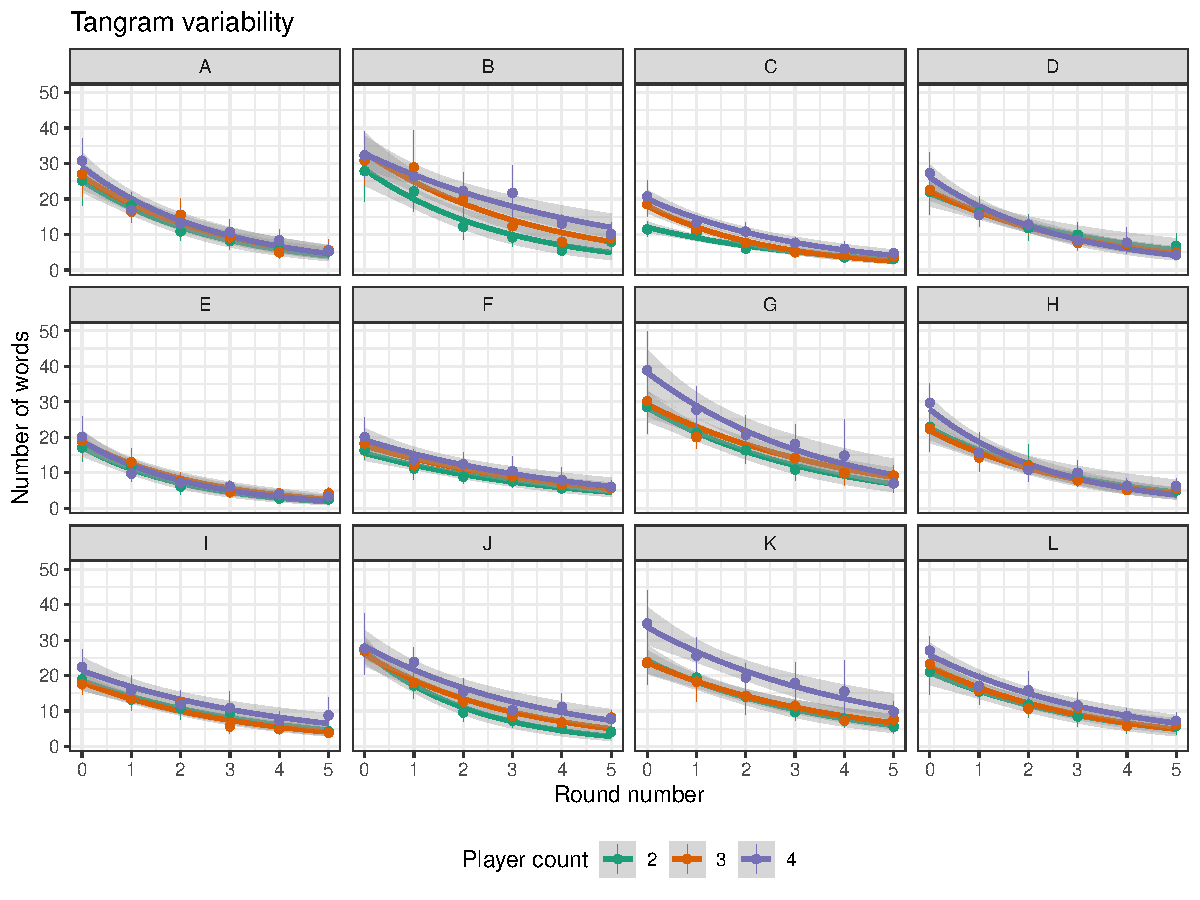
\includegraphics[width=\textwidth]{../images/words_tangrams.pdf}
Tangrams vary in nameability
\end{frame}



\begin{frame}{Planned Analyses}
	\begin{itemize}
		\item Remove chit-chat, model reduction
		\item Semantic convergence in games
		\item Impact of speaker accuracy
	\end{itemize}
\end{frame}


\begin{frame}{Possible future directions}
	Want to understand how references are formed more generally \pause
	
	Possible directions:
\begin{itemize}
	\item Different target images
	\item Curriculum learning
\end{itemize}

\end{frame}

\begin{frame}{Comments, Questions?}
	Looking for feedback on
	\smallskip
	\begin{itemize}
	\item What analyses would be interesting?
	\item What's the next study?
	\end{itemize}
\end{frame}

\appendix


\end{document}

